\documentclass{article}
\usepackage[utf8]{inputenc}

\title{CS 376 Hybrid Systems : HW 8}
\author{Fred Eisele}
\date{19 November 2014}

\usepackage{graphicx}
\usepackage{amsmath}
\usepackage{amsfonts}
\usepackage{xfrac}

\begin{document}

\maketitle

\section{Hybrid Simulation of a Tank Sytem}
Consider the two-tank systems shown in Fig. \ref{fig:two-tanks}.
The system consists of two identical cylindrical tanks,
of unlimited height,
that are connected by a pipe at level $h$.
We denote by $h_1$ and $h_2$ the water levels in
tanks 1 and 2 respectively.
The input flow $Q_{in}$ is provided by a pump and
it is described by

\begin{equation}
Q_{in} = V_{in} k_{in} u(t),
\end{equation}

where $V_{in} \in \{0, 1\}$ represents a valve that can be
used to turn on or off the pump (no partially open valve),
$k_{in}$ is a linear gain, and $u(t)$ is the input
signal representing the flow at the pump.
The flow $Q_a$ between the two tanks is controlled by
a valve $V_a$. An outlet value $V_{out}$ located at the
bottom of tank 2 is used to empty the tank.
Tank 2 is equipped with a sensor that measures the output
flow which is described by

\begin{equation}
Q_{out} = V_{out} k_{out} \sqrt{\rho g h_{2}}
\end{equation}

where $V_{out} \in \{0, 1\}$ represents the outlet valve,
$k_{out}$ is a linear gain, $\rho$ is the density of
the water, and $g$ is the gravitational constant.

\begin{figure}[h!]
\centering
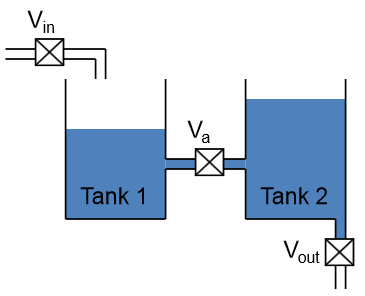
\includegraphics[scale=0.7]{hw8_two_tank_system.png}
\caption{Two-tank system}
\label{fig:two-tanks}
\end{figure}

The dynamic evolution of the systems is described by

\begin{align}
\dot{h_1} & = \frac{1}{A} (Q_{in} - Q_{a}) \\
\dot{h_2} & = \frac{1}{A} (Q_{a} - Q_{a})
\end{align}

where $A$ is the section of the identical cylindrical tanks.
Following Toricelli's law, the flow $Q_{a}$ depends on
the water levels $h_1$ and $h_2$ as follows:

\begin{equation}
Q_{a}  =
 \begin{cases}
 0,        & \mbox{if } h_1 < h \wedge h_2 < h \\
 V_a k_a \sqrt{\rho g (h_1 - h)}, & \mbox{if } h_1 > h \wedge h_2 < h \\
 V_a k_a \sqrt{\rho g (h - h_2)}, & \mbox{if } h_1 < h \wedge h_2 > h \\
 sign(h_1 - h_2) V_a k_a \sqrt{\rho g |h_1 - h_2|}, & \mbox{if } h_1 > h \wedge h_2 > h
\end{cases}  \label{eq:flow-rate-a}
\end{equation}

where $V_a \in \{0, 1\}$ and $k_a$ is a linear gain.
The evolution of the continuous state can be described by

\begin{align}
x & = [h_1, h_2]^T \\
\dot{x} & = f_q(x(t), u(t))
\end{align}

where $q$ is the discrete mode of the sytem.
The mode transitions are based on guard conditions
indicated in Equation \ref{eq:flow-rate-a}.

Assume the following values for the system parameters and initial conditions:

\begin{align}
 V_{in} = V_{a} = V_{out} = 1, & \mbox{  all valves are open} \\
\end{align}

$u(t)$ is a pulse with amplitude $1$ $m^3$ and frequency $1$ $Hz$
resulting in an average rate of $1$ $m^3/sec$.

\begin{align}
 h &= 0.3 \mbox{ m } \\
 k_{in} &= 0.06, \\
 k_{a} &= 0.001, \\
 k_{out} &= 0.001, \\
 g &= 9.81 \mbox{ $m/sec^2$ }, \\
 \rho& = 1000 \mbox{ $kg/m^3$ }, \\
 A &= 0.0154 \mbox{ $m^2$ }
\end{align}


\section{A hybrid automaton model}

The formal model for the two-tank system hybrid automaton.

\begin{equation}
H = (q, X, Init, f, Inv, E, G, R)
\end{equation}

The set of discrete modes.
\begin{align}
 \mbox{if } h_1 < h \wedge h_2 < h, &: separated \\
 \mbox{if } h_1 > h \wedge h_2 < h, &: from_1 \\
 \mbox{if } h_1 < h \wedge h_2 > h, &: from_2 \\
 \mbox{if } h_1 > h \wedge h_2 > h, &: balancing
\end{align}

\begin{equation}
q & = \{ separated, from_1, from_2, balancing \}
\end{equation}

The set of continuous variables.
$X = \mathbb{R}$
\begin{equation}
X = \{ u(t), x, Q_{a}, Q_{out} \}
\end{equation}

The set of initial conditions.
$Init \subseteq Q \times X$
\begin{equation}
Init = \{  \}
\end{equation}

The vector field.
$f: Q \times X$

\begin{equation}
f = f_{separated} \cup f_{from_1} \cup f_{from_2} \cup f_{balancing}
\end{equation}


The invariant set. (all empty)
$Q \mapsto 2^X$

\begin{equation}
Inv = Inv_{separated} \cup Inv_{from_1} \cup Inv_{from_2} \cup Inv_{balancing}
\end{equation}

The invariants are the same for each mode.
$Inv_{i} = $
\begin{align}
  h_1 &\geq 0 \\
  h_2 &\geq 0
\end{align}


$f_{separated} = $
\begin{align}
  Q_{in} &= k_{in} \mbox{ $m/sec^2$ } \\
  Q_a &= 0, \\
  \dot{h_1} &= \frac{Q_{in}}{A} \\
  \dot{h_2} &= -\frac{Q_{out}}{A} \\
  Q_out &= k_{out} \sqrt{\rho g h_2}
\end{align}

$f_{from_1} = $
\begin{align}
  Q_{in} &= k_{in} \mbox{ $m/sec^2$ } \\
  Q_a &= k_{a} \sqrt{\rho g (h_1 - h)}, \\
  \dot{h_1} &= \frac{Q_{in} - Q_a}{A} \\
  \dot{h_2} &= \frac{Q_a - Q_{out}}{A} \\
  Q_out &= k_{out} \sqrt{\rho g h_2}
\end{align}

$f_{from_2} = $
\begin{align}
  Q_{in} &= k_{in} \mbox{ $m/sec^2$ } \\
  Q_a &= k_{a} \sqrt{\rho g (h - h_2)}, \\
  \dot{h_1} &= \frac{Q_{in} - Q_a}{A} \\
  \dot{h_2} &= \frac{Q_a - Q_{out}}{A} \\
  Q_out &= k_{out} \sqrt{\rho g h_2}
\end{align}

$f_{balancing} = $
\begin{align}
  Q_{in} &= k_{in} \mbox{ $m/sec^2$ } \\
  Q_a &= sign(h_1 - h_2) k_a \sqrt{\rho g |h_1 - h_2|} \\
  \dot{h_1} &= \frac{Q_{in} - Q_a}{A} \\
  \dot{h_2} &= \frac{Q_a - Q_{out}}{A} \\
  Q_out &= k_{out} \sqrt{\rho g h_2}
\end{align}

The collection of discrete transitions.
$E \subset Q \times Q$
\begin{align}
E = \{
  & ( separated, from_1 ) \\
  & ( separated, from_2 ) \\
  & ( separated, balanced ) \\
  & ( from_1, separated ) \\
  & ( from_1, from_2 ) \\
  & ( from_1, balanced ) \\
  & ( from_2, from_1 ) \\
  & ( from_2, separated ) \\
  & ( from_2, balanced ) \\
  & ( balanced, from_1 ) \\
  & ( balanced, from_2 ) \\
  & ( balanced, separated )  \}
\end{align}

The guards on the transitions.
$G: E \mapsto 2^X$
\begin{align}
E = \{
  & ( separated, from_1 ), h_1 > h \wedge h_2 < h, \\
  & ( separated, from_2 ), h_1 < h \wedge h2 > h, \\
  & ( separated, balanced ), h_1 > h \wedge h_2 > h, \\
  & ( from_1, separated ), h_1 < h \wedge h_2 < h, \\
  & ( from_1, from_2 ), h_1 < h \wedge h2 > h, \\
  & ( from_1, balanced ), h_1 > h \wedge h_2 > h,  \\
  & ( from_2, from_1 ), h_1 > h \wedge h_2 < h, \\
  & ( from_2, separated ), h_1 < h \wedge h_2 < h, \\
  & ( from_2, balanced ), h_1 > h \wedge h_2 > h,  \\
  & ( balanced, from_1 ), h_1 > h \wedge h_2 < h, \\
  & ( balanced, from_2 ), h_1 < h \wedge h2 > h, \\
  & ( balanced, separated ), h_1 < h \wedge h_2 < h,  \}
\end{align}

The reset relation on the transitions.
$R: E \times X \mapsto 2^X$
\begin{align}
R = \emptyset
\end{align}

\section{Simulink Simulation}

\begin{figure}[h!]
\centering
\includegraphics[scale=0.7]{hw8_two_tank_model.png}
\caption{Two-tank SimuLink Model}
\label{fig:two-tank-model}
\end{figure}

The model is simulated for several initial conditions $x_0 = [h_1, h_2]^T$.
The continuous state $Q_{a}, x$, discrete state $q$, and
output $Q_{out}$ of the system are plotted.

\subsection{$x_0 = [0.20, 0.75]^T$}

\begin{figure}[h!]
\centering
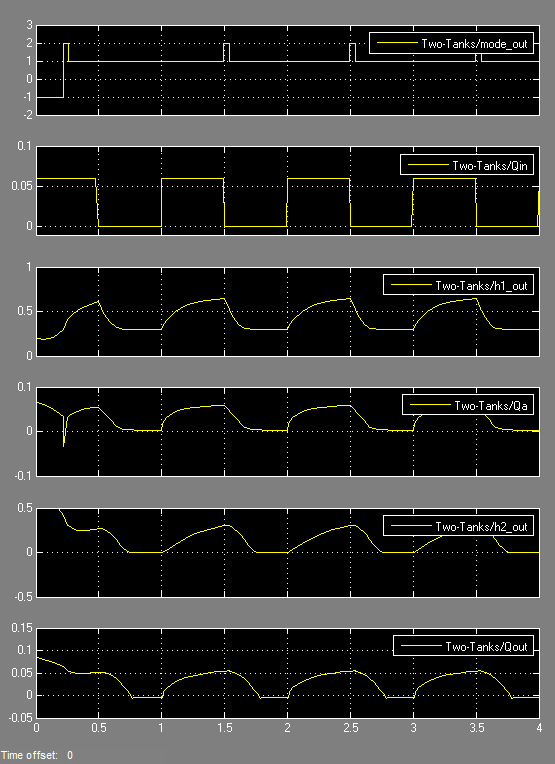
\includegraphics[scale=0.7]{hw8_20_75.png}
\caption{Two-tank SimuLink Model, $x_0 = [0.2, 0.75]^T$ }
\label{fig:two-tank-model-20-75}
\end{figure}

\subsection{$x_0 = [0.50, 0.20]^T$}

\begin{figure}[h!]
\centering
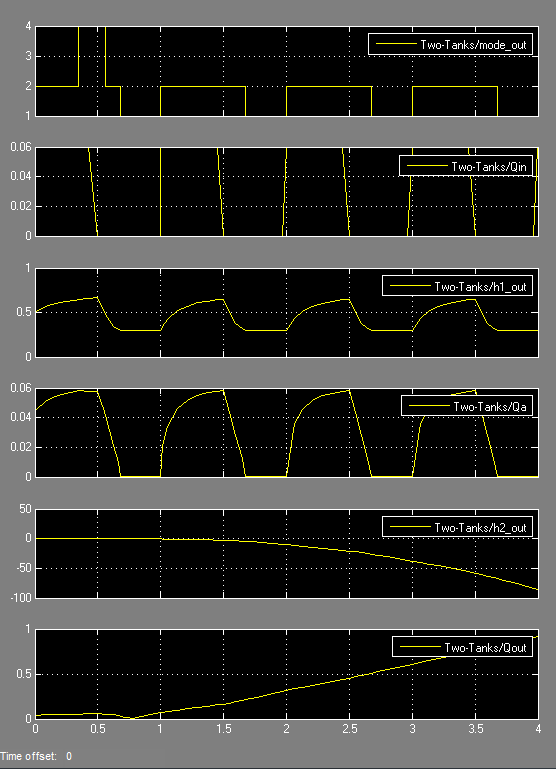
\includegraphics[scale=0.7]{hw8_50_20.png}
\caption{Two-tank SimuLink Model, $x_0 = [0.50, 0.20]^T$ }
\label{fig:two-tank-model-50-20}
\end{figure}

\subsection{$x_0 = [0.50, 0.50]^T$}

\begin{figure}[h!]
\centering
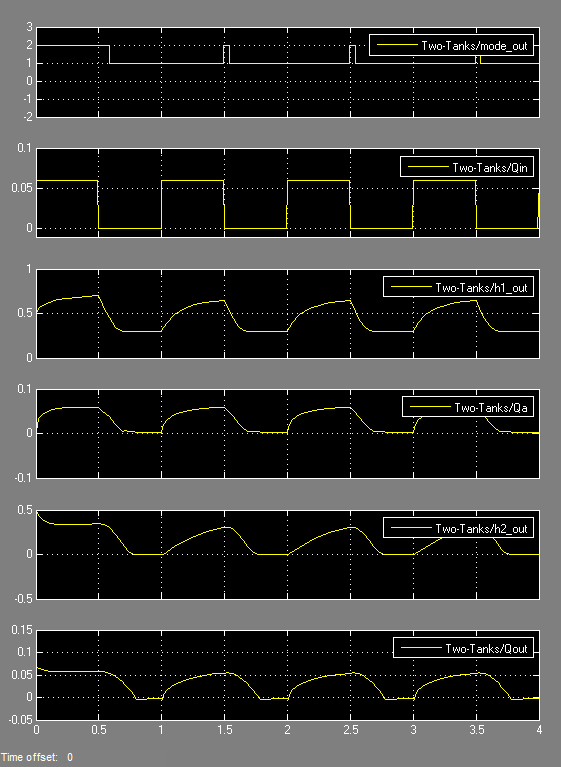
\includegraphics[scale=0.7]{hw8_50_50.png}
\caption{Two-tank SimuLink Model, $x_0 = [0.50, 0.50]^T$ }
\label{fig:two-tank-model-50-50}
\end{figure}

\subsection{$x_0 = [0.20, 0.20]^T$}

\begin{figure}[h!]
\centering
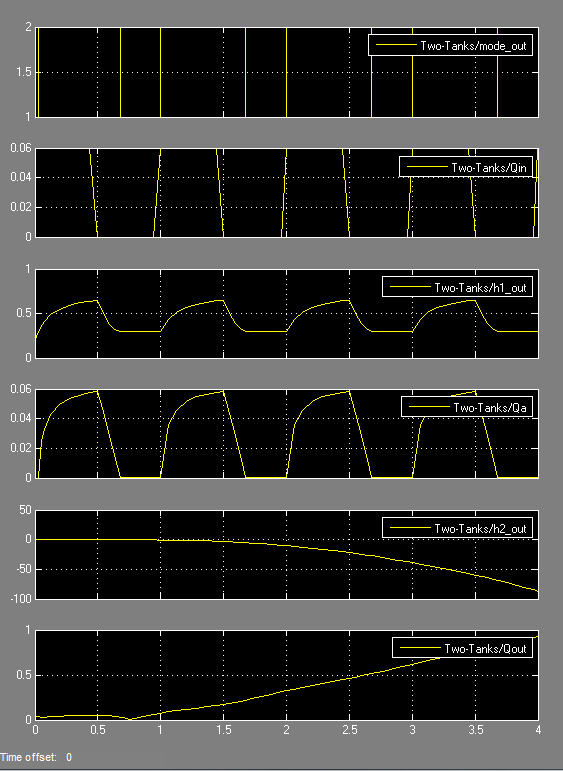
\includegraphics[scale=0.7]{hw8_20_20.png}
\caption{Two-tank SimuLink Model, $x_0 = [0.20, 0.20]^T$ }
\label{fig:two-tank-model-20-20}
\end{figure}

\end{document}
